
\section{Data visualization using PCA}

As we can see from Figure~\ref{fig:PCA_2D} and Figure~\ref{fig:PCA_3D}, the dataset is highly imbalanced, with Class 0 dominating. There's no clear separation between most of the data points and a few outliers. \textbf{However, we cannot conclude any definitive information because this is just a projection in low dimension.}




\begin{figure}[h]
    \centering
    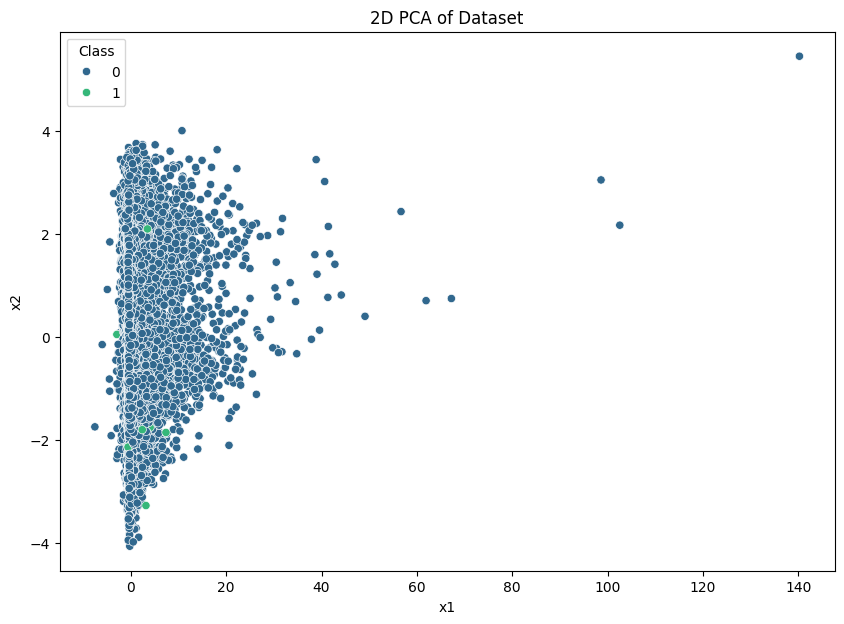
\includegraphics[width=0.5\linewidth]{PCA_2D.png}
    \caption{2D PCA of Dataset}
    \label{fig:PCA_2D}
\end{figure}


\begin{figure}[h]
    \centering
    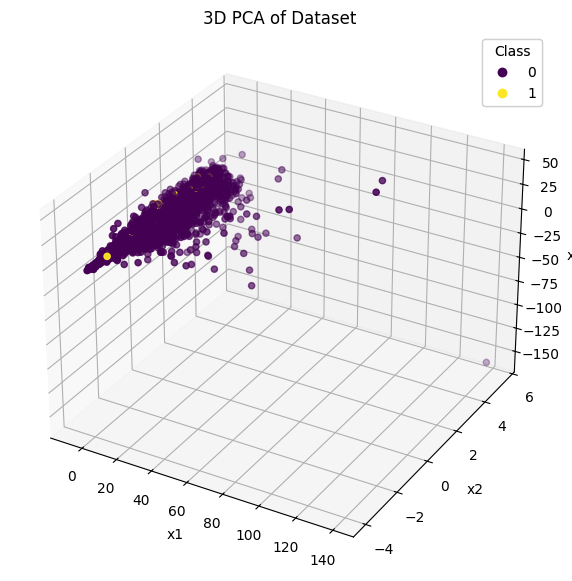
\includegraphics[width=0.5\linewidth]{3D PCA of Dataset.png}
    \caption{3D PCA of Dataset}
    \label{fig:PCA_3D}
\end{figure}